\documentclass{article}
\usepackage{graphicx}
\usepackage{amsmath}
\usepackage{amssymb}
\usepackage[a4paper, top=25mm, bottom=25mm, left=25mm, right=25mm]{geometry}
\usepackage{pgfplots}
\pgfplotsset{compat=1.18}
\usepackage{mathtools}

\begin{document}
\pagestyle{empty}
\large

\begin{center}
2023-2024 Spring \\MAT124 Midterm\\(26/04/2024)
\end{center}

\noindent 1. Sketch the traces of the following surfaces with the coordinate planes $x=0,\:y=0$, and $z=0$, and then sketch the graphs of them.

\hfill

\noindent (a) $y=\ln z$ \ \ \ (b) $x^2+2y^2-3z^2+1=0$

\hfill

\noindent 2. State the $\epsilon-\delta$ definition of the limit of a function of two variables, and using the $\epsilon-\delta$ definition, show that
\[\lim_{(x,y)\to(0,0)}\left(2x^2+y^2\right)=0\]

\hfill

\noindent 3. For $t\in\mathbb{R}$, let $l_1$ and $l_2$ be two lines given by

\[\begin{array}{ccccc}
x=3t&&&x=1+6\lambda&\\
y=4-t&t\in\mathbb{R}&& y=2-2\lambda&\lambda\in\mathbb{R}\\
z=1+2t&&\qquad&z=1+4\lambda&
\end{array}\]

\hfill

\noindent Determine an equation of the plane containing both $l_1$ and $l_2$.

\hfill

\noindent 4. Let
\[f(x,y)=\left\{\begin{array}{cc}
\displaystyle\frac{x^2\cdot\mathrm{e}^{x^2+y}}{x^2+y^2}&\text{if }(x,y)\neq(0,0)\\[1em]
0&\text{if }(x,y)=(0,0)
\end{array}\right.\]

\hfill

\noindent (i) Evaluate the partial derivatives $f_x(0,0)$ and $f_y(0,0)$.

\hfill

\noindent (ii) Show that $f(x,y)$ is not differentiable at $(0,0)$.

\hfill

\noindent 5. Let $u=u(x,y)$ and $v=v(x,y)$. The Cauchy-Riemann equations are

\[\frac{\partial u}{\partial x}=\frac{\partial v}{\partial y}\quad\text{and}\quad\frac{\partial u}{\partial y}=-\frac{\partial v}{\partial x}\]

\noindent Show that in the polar coordinate system $(x=r\cos\theta,\:y=r\sin\theta)$,

\[\frac{\partial u}{\partial r}=\frac1r\frac{\partial v}{\partial\theta}\quad\text{and}\quad\frac{\partial v}{\partial r}=-\frac1r\frac{\partial u}{\partial \theta}\]

\hfill

\noindent 6. Determine the direction at the point $(1,1)$ in which the rate of change of

\[f(x,y)=\frac{2^{xy}}x\]

\hfill

\noindent is the largest. Compute this rate of change.

\hfill

\noindent 7. Find all critical points of the function

\[f(x,y)=(x-1)(y+1)(x-y+3)\]

\hfill

\noindent and then determine whether each critical point corresponds to a local maximum, a local minimum or a saddle point.

\newpage

\begin{center}
2023-2024 Spring Midterm (26/04/2024) Solutions\\
(Last update: 8/27/25 (27th of August) 11:24 PM)
\end{center}

\noindent 1.

\hfill

\noindent (a)
\begin{center}
\begin{tikzpicture}
  \begin{axis}[
  title={Plane $x=0$},
    xlabel=$y$, ylabel=$z$,
    xtick=\empty, ytick=\empty,
    samples=30,
    axis lines=middle,
    clip=true,
    scale=1,
    enlargelimits=true
    ]
    \addplot[domain=-1:0.8, blue] {e^x};

    \node[blue] at (0.5,1) {$z=\mathrm{e}^y$};
  \end{axis}
\end{tikzpicture}\hspace{1em}
\begin{tikzpicture}
  \begin{axis}[
  title={Plane $y=0$},
    xlabel=$x$, ylabel=$z$,
    xtick=\empty, ytick=\empty,
    axis lines=middle,
    samples=30,
    clip=true,
    ymin=0, ymax=2,
    scale=1,
    enlargelimits=true
    ]
    \addplot[domain=-2:2, red, thick] {1};

    \node[red] at (1.5,1.5) {$z=1$};
  \end{axis}
\end{tikzpicture}

\hfill

\begin{tikzpicture}
  \begin{axis}[
  title={Plane $z=0$ (No intersection)},
  axis equal image,
    xlabel=$x$, ylabel=$y$,
    xtick=\empty, ytick=\empty,
    xmin=-1, xmax=1,
    ymin=-1, ymax=1,
    axis lines=center,
    clip=true,
    scale=1,
    enlargelimits=true
    ]
  \end{axis}
\end{tikzpicture}\hspace{1em}
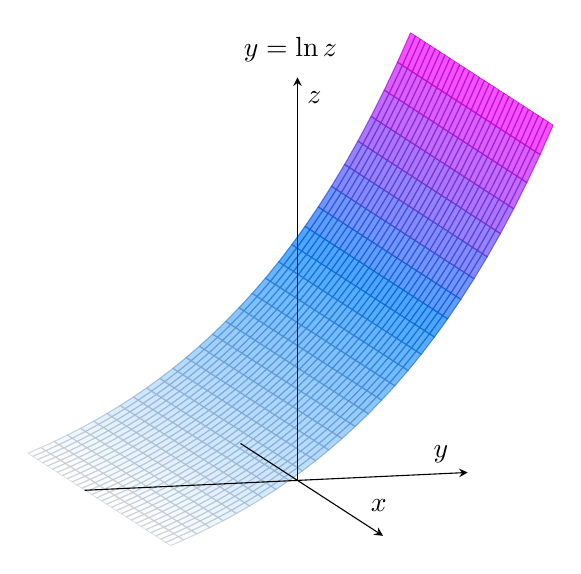
\begin{tikzpicture}
  \begin{axis}[
    title={$y=\ln z$},
    title style={yshift=-20pt},
      view={75}{10},
      axis lines=center,
      axis equal image,
      xlabel={$x$},
      ylabel={$y$},
      zlabel={$z$},
      domain=-1:1.5,
      y domain=-1:0.8,
      samples=30,
      samples y=30,
      colormap/cool,
      axis on top,
      scale=1.25,
      xtick=\empty, ytick=\empty, ztick=\empty,
      z buffer=sort,
    ]
    \addplot3[
      surf,
      opacity=0.7
    ]
    ( {x},
      {y},
      {e^y} );
  \end{axis}
\end{tikzpicture}
\end{center}

\hfill

\noindent (b)
\begin{center}
\begin{tikzpicture}
  \begin{axis}[
  title={Plane $x=0$},
    xlabel=$y$, ylabel=$z$,
    xtick=\empty, ytick=\empty,
    samples=30,
    axis lines=middle,
    clip=true,
    scale=1,
    enlargelimits=true
    ]
    \addplot[domain=-2:2, blue] {sqrt(2*x^2/3+1/3)};
    \addplot[domain=-2:2, blue] {-sqrt(2*x^2/3+1/3)};
    
    \node[blue] at (1.25,-0.4) {$2y^2+1=3z^2$};
  \end{axis}
\end{tikzpicture}\hspace{1em}
\begin{tikzpicture}
  \begin{axis}[
  title={Plane $y=0$},
    xlabel=$x$, ylabel=$z$,
    xtick=\empty, ytick=\empty,
    samples=30,
    axis lines=middle,
    clip=true,
    scale=1,
    enlargelimits=true
    ]
    \addplot[domain=-2:2, red] {sqrt(x^2/3+1/3)};
    \addplot[domain=-2:2, red] {-sqrt(x^2/3+1/3)};
    
    \node[red] at (1.25,-0.4) {$x^2+1=3z^2$};
  \end{axis}
\end{tikzpicture}

\begin{tikzpicture}
  \begin{axis}[
  title={Plane $z=0$ (No intersection)},
  axis equal image,
    xlabel=$x$, ylabel=$y$,
    xtick=\empty, ytick=\empty,
    xmin=-1, xmax=1,
    ymin=-1, ymax=1,
    axis lines=center,
    clip=true,
    scale=1,
    enlargelimits=true
    ]
  \end{axis}
\end{tikzpicture}\hspace{1em}
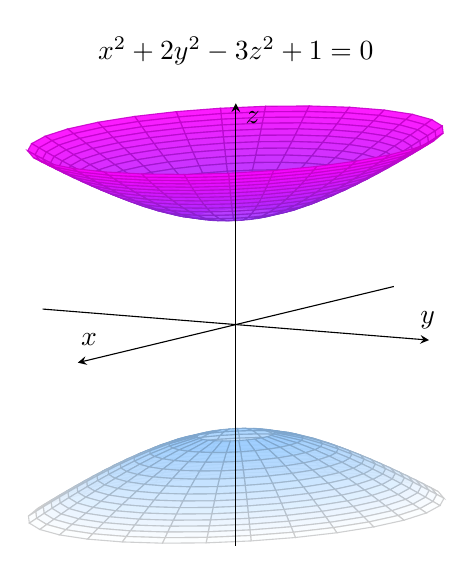
\begin{tikzpicture}
  \begin{axis}[
  title={$x^2+2y^2-3z^2+1=0$},
    title style={yshift=-15pt},
      view={120}{8},
      axis lines=center,
      axis equal image,
      xlabel={$x$},
      ylabel={$y$},
      zlabel={$z$},
      domain=0:2*pi,
      y domain=-2:2,
      samples=30,
      samples y=30,
      colormap/cool,
      axis on top,
      scale=1.6,
      xtick=\empty, ytick=\empty, ztick=\empty,
      z buffer=sort,
      enlargelimits=true,
    ]
    \addplot3[
      surf,
      opacity=0.9
    ]
    ( {sqrt(y)*cos(deg(x))},
      {1/sqrt(2))*sqrt(y)*sin(deg(x))},
      {(1/sqrt(3))*sqrt(y+1)} );
    \addplot3[
      surf,
      opacity=0.9
    ]
    ( {-sqrt(y)*cos(deg(x))},
      {-1/sqrt(2))*sqrt(y)*sin(deg(x))},
      {-(1/sqrt(3))*sqrt(y+1)} );
  \end{axis}
\end{tikzpicture}
\end{center}

\hfill

\noindent 2. The $\epsilon-\delta$ definition is the formal way of calculating the limit of a function at a point $(x_0,y_0)$. According to the definition, for every $\epsilon>0$, there exists a $\delta$ such that

\[0<\sqrt{(x-x_0)^2+(y-y_0)^2}<\delta\implies\left|f(x,y)-L\right|<\epsilon,\]

\hfill

\noindent where $L$ is the limit.

\hfill

\noindent Then for every $\epsilon>0$, there exists a $\delta$ such that

\[0<\sqrt{x^2+y^2}<\delta\implies\left|2x^2+y^2\right|<\epsilon.\]

\[\left|2x^2+y^2\right|\leq2x^2+y^2\qquad\left[x^2\geq0,\quad y^2\geq0\right]\]

\[2x^2+y^2\leq2x^2+2y^2=2\left(x^2+y^2\right)\leq2\delta^2\qquad\left[\sqrt{x^2+y^2}<\delta\implies  x^2+y^2<\delta^2\right]\]

\hfill

\noindent Let $\delta=\sqrt{\dfrac{\epsilon}2}$.

\[\left|2x^2+y^2\right|\leq2\left(x^2+y^2\right)<2\cdot\left(\sqrt{\frac{\epsilon}2}\right)^2=2\cdot\frac{\epsilon}2=\epsilon\]

\hfill

\noindent This shows that the limit is equal to $0$.

\hfill

\noindent 3. The coefficients of the parametrization variables have the same ratio. That is, they are parallel. Choose $P_1(3,3,3)$ on $l_1$ and $P_2(1,2,1)$ on $l_2$. The cross product of $\mathbf u=\left\langle3,-1,2\right\rangle$, which is parallel to the lines, and the vector $\mathbf v$ joining $P_1$ and $P_2$, where $\mathbf w=\left\langle3-1,\,3-2,\,3-1\right\rangle=\left\langle2,1,2\right\rangle$, gives us the normal of the plane.

\begin{align*}\mathbf n&=\mathbf{u}\times\mathbf{v}=\left|\begin{array}{ccc}
\mathbf{i}&\mathbf{j}&\mathbf{k}\\
3&-1&2\\
2&1&2
\end{array}\right|=\mathbf{i}\left|\begin{array}{cc}
-1&2\\1&2
\end{array}\right|-\mathbf{j}\left|\begin{array}{cc}
3&2\\2&2
\end{array}\right|+\mathbf{k}\left|\begin{array}{cc}
3&-1\\2&1
\end{array}\right|\\\\&=(-1\cdot2-1\cdot2)\mathbf{i}-(3\cdot2-2\cdot2)\mathbf{j}+(3\cdot1-2\cdot(-1))\mathbf{k}=-4\mathbf i-2\mathbf j+5\mathbf k\end{align*}

\hfill

\noindent Using the definition $\mathbf{n}\cdot\overrightarrow{PP_1}=0$, where $P$ is a point on the plane, the equation of the plane is

\begin{align*}\mathbf{n}\cdot\overrightarrow{PP_1}=0&\implies\left\langle-4,-2,5\right\rangle\cdot\left\langle x-3,\,y-3,\,z-3\right\rangle=0\\\\&\implies-4(x-3)-2(y-3)+5(z-3)=0\implies\boxed{-4x-2y+5z+3=0}\end{align*}

\hfill

\noindent 4.

\hfill

\noindent (i) Use the definition of the partial derivative.

\begin{align*}f_x|_{(0,0)}&=\lim_{h\to0}\frac{f(0+h,0)-f(0,0)}h=\lim_{h\to0}\frac{\dfrac{(0+h)^2\cdot\mathrm{e}^{(0+h)^2+0}}{(0+h)^2+0^2}}{h}=\lim_{h\to0}\frac{\mathrm{e}^{h^2}}{h}\\\\&=\infty\:(f_x\:\text{does not exist})\end{align*}

\[f_y|_{(0,0)}=\lim_{h\to0}\frac{f(0,0+h)-f(0,0)}h=\lim_{h\to0}\frac{\dfrac{0^2\cdot\mathrm{e}^{0^2+(0+h)}}{0^2+(0+h)^2}}{h}=\lim_{h\to0}\frac{0}{h}=0\]

\hfill

\noindent (ii) $f_y$ is a finite number. However, since $f_x$ does not exist, $f$ is not differentiable at $(0,0)$.

\hfill

\noindent 5. $u$ and $v$ are functions of $x$ and $y$. $x$ and $y$ are functions of $r$ and $\theta$. Use the chain rule.

\[\frac{\partial u}{\partial r}=\frac{\partial u}{\partial x}\cdot\frac{\partial x}{\partial r}+\frac{\partial u}{\partial y}\cdot\frac{\partial y}{\partial r}=u_x\cdot\cos\theta+u_y\cdot\sin\theta=v_y\cos\theta-v_x\sin\theta\]

\[\frac{\partial v}{\partial\theta}=\frac{\partial v}{\partial x}\cdot\frac{\partial x}{\partial\theta}+\frac{\partial v}{\partial y}\cdot\frac{\partial y}{\partial\theta}\implies\frac1r\frac{\partial v}{\partial\theta}=\frac1r\left(-v_x\cdot r\sin\theta+v_y\cdot r\cos\theta\right)=-v_x\sin\theta+v_y\cos\theta\]

\[\frac{\partial u}{\partial r}=-v_x\sin\theta+v_y\cos\theta=\frac1r\frac{\partial v}{\partial\theta}\]

\hfill

\[\frac{\partial v}{\partial r}=\frac{\partial v}{\partial x}\cdot\frac{\partial x}{\partial r}+\frac{\partial v}{\partial y}\cdot\frac{\partial y}{\partial r}=v_x\cdot\cos\theta+v_y\cdot\sin\theta=-u_y\cos\theta+u_x\sin\theta\]

\[\frac{\partial u}{\partial\theta}=\frac{\partial u}{\partial x}\cdot\frac{\partial x}{\partial\theta}+\frac{\partial u}{\partial y}\cdot\frac{\partial y}{\partial\theta}\implies-\frac1r\frac{\partial u}{\partial\theta}=-\frac1r\left(-u_x r\sin\theta+u_y r\cos\theta\right)=u_x\sin\theta-u_y\cos\theta\]

\[\frac{\partial v}{\partial r}=u_x\sin\theta-u_y\cos\theta=-\frac1r\frac{\partial u}{\partial \theta}\]

\hfill

\noindent 6. The function $f$ has the maximum rate of change if the gradient vector of $f$ and the unit direction vector $\mathbf u$ are in the same direction. Apply the quotient rule to compute the gradient of $f$.
\[\nabla f=\left\langle\frac{\left(2^{xy}\cdot y\cdot\ln2\right)\cdot x-2^{xy}\cdot(1)}{x^2},\,2^{xy}\cdot\ln2\right\rangle=\left\langle\frac{2^{xy}\left(yx\ln2-1\right)}{x^2},\,2^{xy}\cdot\ln2\right\rangle\]

\[\left(\nabla f\cdot\mathbf u\right)_{\text{max}}=\left|\nabla f\right||u|\cos0=|\nabla f|\]

\begin{align*}\nabla f|_{(1,1)}&=\left\langle2\ln2-2,\,2\ln2\right\rangle\implies|\nabla f|=\sqrt{\left(2\ln2-2\right)^2+\left(2\ln2\right)^2}\\\\&=2\sqrt{2\ln^22-2\ln2+1}\end{align*}

\hfill

\noindent The unit direction vector $u$ is
\[\mathbf{u}=\frac{\nabla f}{|\nabla f|}=\frac{\left\langle2\ln2-2,\,2\ln2\right\rangle}{2\sqrt{2\ln^22-2\ln2+1}}=\left\langle\frac{\ln2-1}{\sqrt{2\ln^22-2\ln2+1}},\frac{\ln2}{\sqrt{2\ln^22-2\ln2+1}}\right\rangle\]

\[\boxed{\begin{array}{c}\text{The maximum rate of change: }{2\sqrt{2\ln^22-2\ln2+1}}\\[1em]\text{The direction vector:}\left\langle\dfrac{\ln2-1}{\sqrt{2\ln^22-2\ln2+1}},\dfrac{\ln2}{\sqrt{2\ln^22-2\ln2+1}}\right\rangle\end{array}}\]

\hfill

\noindent 7. Apply the chain rule.
\begin{align*}f_x&=(y+1)\left[1\cdot(x-y+3)+(x-1)\cdot1\right]=(y+1)(2x-y+2)\\\\&=2xy-y^2+2y+2x-y+2=-y^2+y+2xy+2x+2\end{align*}
\begin{align*}f_y&=(x-1)\left[1\cdot(x-y+3)+(y+1)\cdot(-1)\right]=(x-1)(x-2y+2)\\\\&=x^2-2xy+2x-x+2y-2=x^2-2xy+x+2y-2\end{align*}

\hfill

\noindent The critical points occur where one of the partial derivatives does not exist or $f_x=f_y=0$. $f_x$ and $f_y$ are continuous everywhere. Therefore, we may simply determine where $f_x=f_y=0$.

\begin{align*}f_x=f_y=0&\implies\left.\begin{array}{rc}
2xy-y^2+2y+2x-y+2=0&(1)\\
x^2-2xy+x+2y-2=0
\end{array}\right\}\quad x^2-y^2+3(x+y)=0\\\\&\implies(x-y)(x+y)+3(x+y)=0\implies(x-y+3)(x+y)=0\end{align*}

\hfill

\noindent We have two cases: $x+3=y$ or $x=-y$.

\begin{flalign*}\text{Case I}:x=-y&\overset{(1)}\implies-y^2-2y^2+y-2y+2=0\implies -3y^2-y+2=0\\\\&\implies
(2-3y)(y+1)=0\implies y_1=\frac23,\:y_2=-1&\end{flalign*}
\[y_1=\frac23\implies x_1=-\frac23\qquad y_2=-1\implies x_2=1\]

\begin{flalign*}\text{Case II}:x+3=y&\overset{(1)}\implies-(x+3)^2+2x(x+3)+x+3+2x+2=0\\\\&\implies-x^2-6x-9+2x^2+6x+3x+5=0\implies x^2+3x-4=0&\end{flalign*}
\[x_{3,4}=\frac{-3\pm\sqrt{9-4\cdot1\cdot(-4)}}{2\cdot1}=\frac{-3\pm5}2\implies x_3=-4,\:x_4=1\implies y_3=-1,\:y_4=4\]

\hfill

\noindent To classify these four critical points, apply the Second Derivative Test.

\[f_{xx}=2y+2,\quad f_{xy}=f_{yx}=2x-2y+1,\quad f_{yy}=-2x+2\]

\begin{flalign*}\left(-\frac23,\frac23\right)\rightarrow\left\{\:\begin{array}{l}
f_{xx}=\dfrac{10}3,\quad f_{xy}=-\dfrac53 ,\quad f_{yy}=\dfrac{10}3\\[1em]
\left|\begin{array}{cc}
\dfrac{10}3&-\dfrac{10}3\\[1em]
-\dfrac53 & \dfrac{10}3
\end{array}\right|=\dfrac{10}3\cdot\dfrac{10}3-\left(-\dfrac53\right)\cdot\left(-\dfrac53\right)=\dfrac{25}3,\quad f_{xx}=\dfrac{10}3>0
\end{array}\right.&&\end{flalign*}

\begin{flalign*}\left(1,-1\right)\rightarrow\left\{\:\begin{array}{l}
f_{xx}=0,\quad f_{xy}=5,\quad f_{yy}=0\\[1em]
\left|\begin{array}{cc}
0 & 5\\
5 & 0
\end{array}\right|=0\cdot0-5\cdot5=-25<0
\end{array}\right.&&\end{flalign*}

\begin{flalign*}\left(-4,-1\right)\rightarrow\left\{\:\begin{array}{l}
f_{xx}=0,\quad f_{xy}=-5,\quad f_{yy}=10\\[1em]
\left|\begin{array}{cc}
0 & -5\\
-5 & 10
\end{array}\right|=0\cdot10-(-5)\cdot(-5)=-25<0
\end{array}\right.&&\end{flalign*}

\begin{flalign*}\left(1,4\right)\rightarrow\left\{\:\begin{array}{l}
f_{xx}=10,\quad f_{xy}=5,\quad f_{yy}=0\\[1em]
\left|\begin{array}{cc}
10 & 5\\
5 & 0
\end{array}\right|=10\cdot0-5\cdot5=-25<0
\end{array}\right.&&\end{flalign*}

\[\boxed{\begin{array}{c}\text{A local minimum occurs at }\left(-\dfrac23,\dfrac23\right).\\\text{ Saddle points occur at } (1,-1), (-4,-1),\:\text{and}\:(1,4).\end{array}}\]

\end{document}